\section{Background}

This study presents character recognition within the context of short, alphanumeric number sequences. We define alphanumeric number sequences as short fragments of digits within an unstructured scene.   

Certain literature have focused on these kinds of sequences, namely: License Plate Recognition (LPR\newacronym{lpr}{LPR}{Licence Plate Recognition}) systems \citep{CanoPerez:2003fq,Anagnostopoulos:2006wv}; Traffic Sign Recognition (TSR\newacronym{tsr}{TSR}{Traffic Sign Recognition}), namely speed limit recognition, to better realise Advanced Driver Assistance Systems (ADAS\newacronym{adas}{ADAS}{Advanced Driver Assistance Systems}) \citep{Eichner:2008dw,Kundu:2015vq,Seo:2015ez,Lian:2016dc}; and, street number recognition, specifically a study by \citet{Netzer:2011to}, using Google Street View\footnoteurl{https://www.google.com/streetview/}{13 May 2017} to determine the numerical value of street numbers. Figure~\ref{fig:sample_sequences} summarises the usage of these sequences.

Different applications apply varying methods to parse short alphanumeric characters. There are typically two stages of any parsing method: detection of possible candidates and recognition of the text itself. Detection techniques usually are categorised as either connected component (CC)\newacronym{cc}{CC}{Connected Component}-based or learning or texture-based. CC-based detection will typically use a set of distinct properties on the image to detect relevant areas (such as width, stroke and colour) while learning-based feed images into a classifier that can distinguish candidates from false positives. The recognition phase can typically be achieved using optical image recognition OCR engines, machine learning algorithms or deep neural networks to classify the detected regions.

{
  \itshape
  This study proposes the development of a learning-based detection and recognition pipeline using deep-learning neural networks within the context of unstructured photos, namely focusing within the context of marathon Racing Bib Numbers (RBNs)\newacronym{rbn}{RBN}{Racing Bib Number}, as shown in Figure~\ref{fig:sample_rbns}.
}

\begin{figure}[tbh!]
  \centering
  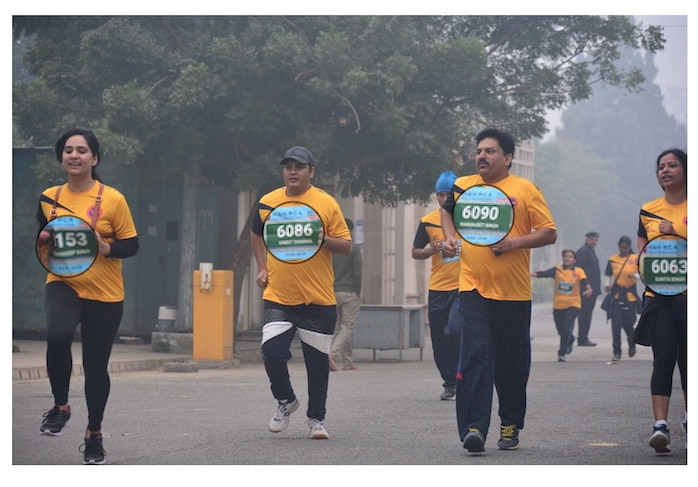
\includegraphics[width=0.8\textwidth]{images/introduction/rbn}
  \caption[Sample racing bib numbers]{Four RBNs in a sample marathon photo.}
  \label{fig:sample_rbns}
\end{figure}

\begin{figure}
  \centering
  \begin{subfigure}[b]{0.45\textwidth}
    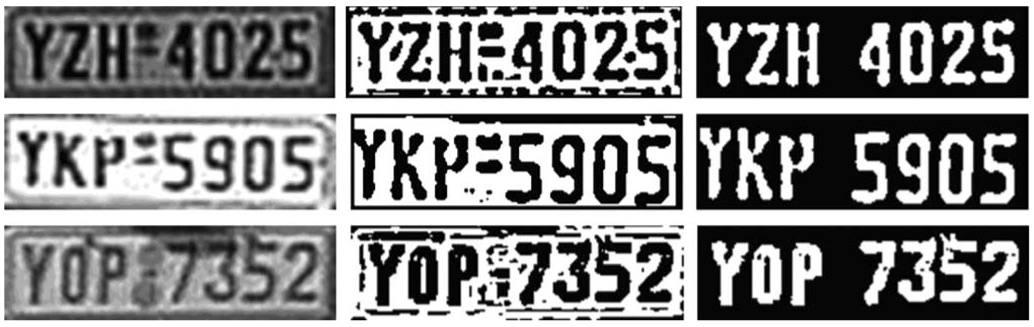
\includegraphics[width=\textwidth]{images/introduction/lpr}
    \caption{Successful character segmentation using the LPR method described by \citet{Anagnostopoulos:2006wv}. From left to right: original image, region segmentation, character segmentation after negation, height and orientation measurements.}
  \end{subfigure}
  \hspace{0.05\textwidth}
  \begin{subfigure}[b]{0.45\textwidth}
    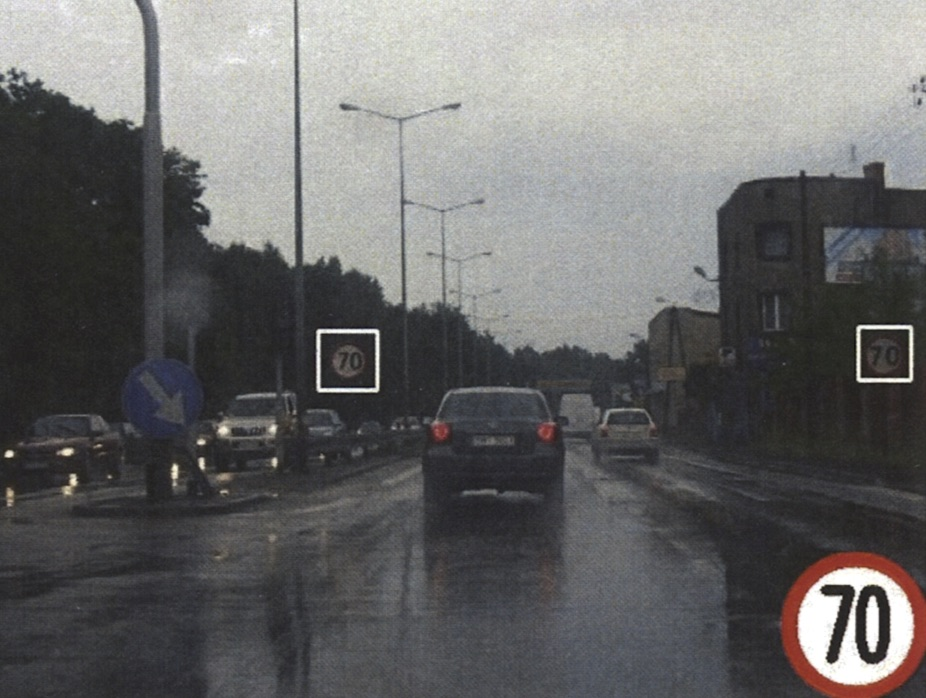
\includegraphics[width=\textwidth]{images/introduction/tsr}
    \caption{Successful recognition of speed sign digits shown in \citet{Eichner:2008dw}.}
  \end{subfigure}\\
  \vspace{1cm}
  \begin{subfigure}[b]{0.45\textwidth}
    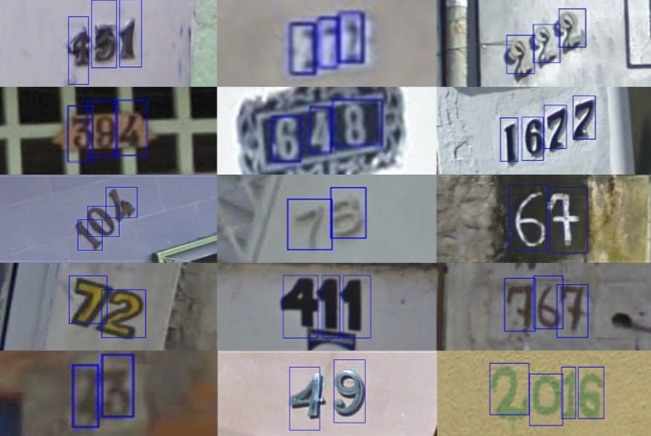
\includegraphics[width=\textwidth]{images/introduction/streetview}
    \caption{Localisation of digits found from varying street view house numbers using the worker described in \citet{Eichner:2008dw}.}
  \end{subfigure} 
  \caption{Various sample alphanumeric sequences observed in literature.}
  \label{fig:sample_sequences}
\end{figure}